\subsection{Time dependent coordinate transformation}
wave equation

\subsection{orbital parameters (osculating orbits paper)}

\begin{figure}
  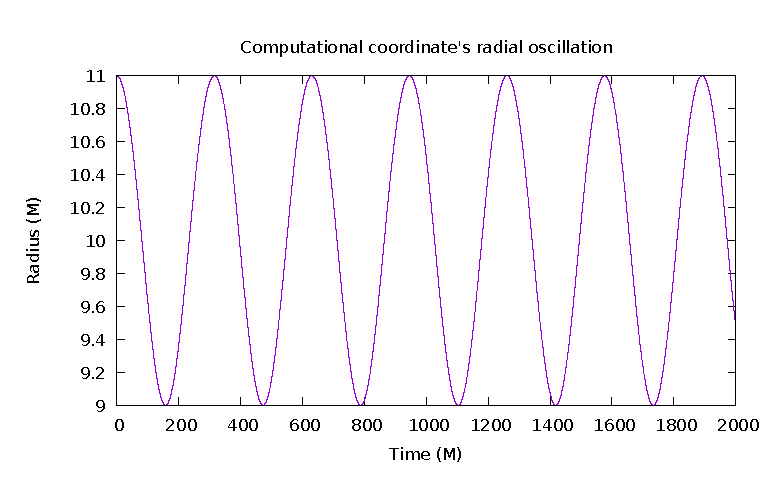
\includegraphics{orbit}
  \caption{Schwarszchild r as a function of time over several orbits.}
\end{figure}

\begin{figure}
  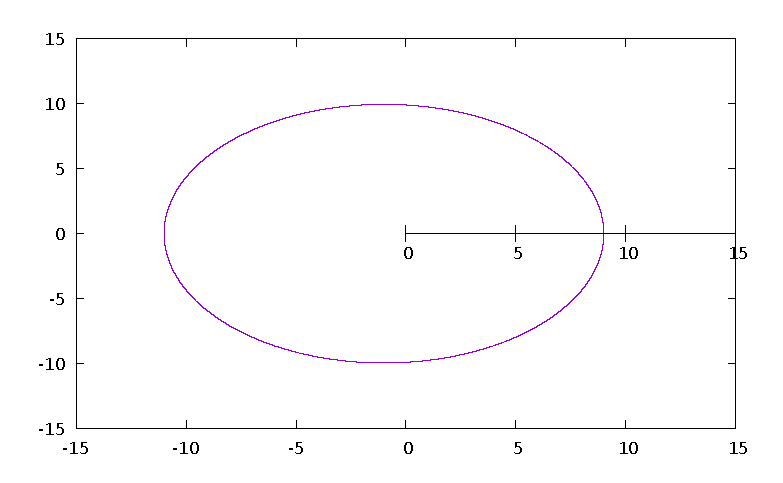
\includegraphics{orbitdg44p99e01}
  \caption{Plotting $\chi$ as the angle in polar coordinates, the orbit forms an exact ellipse. This is the definition of $\chi$, provided r is in Schwarzschild coordinates. Shown for $p=9.9$ and $e=0.1$, DG order 44}
\end{figure}

\begin{figure}
  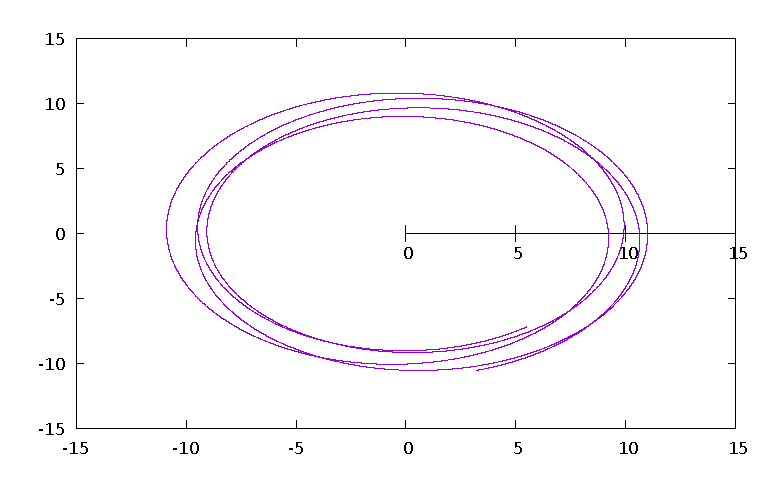
\includegraphics{orbitevolvedg44p99e01}
  \caption{Plotting the orbit as it physically would exist, using Schwarzschild $\phi$ as the polar coordinate angle, the orbit precesses but does not inspiral since there is no generic evolution yet. Shown for $p=9.9$ and $e=0.1$, DG order 44}
\end{figure}


\begin{figure}
  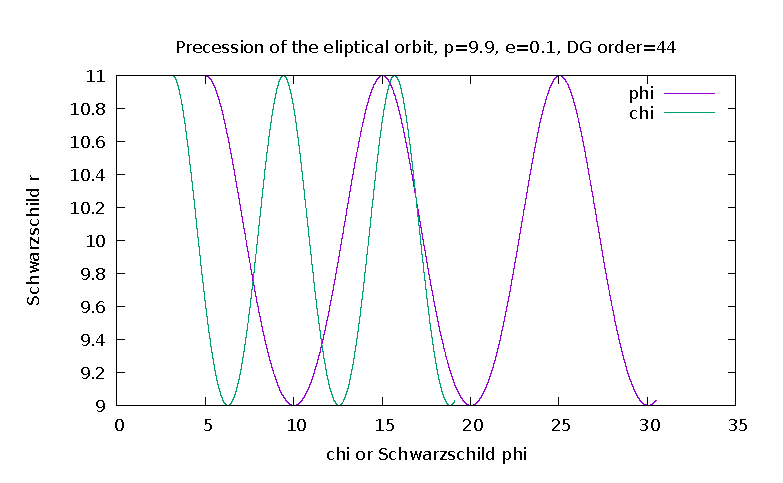
\includegraphics{precessiondg44p99e01}
  \caption{Precession of the eliptical orbit is demonstrated due to the inequality in the period of the angular variables $\chi$, which represents the period of the radial oscillations, and $\phi$, which represents the period of the angular oscillations. $p=9.9$, $e=0.1$, DG order 44.}
\end{figure}



\begin{figure}
  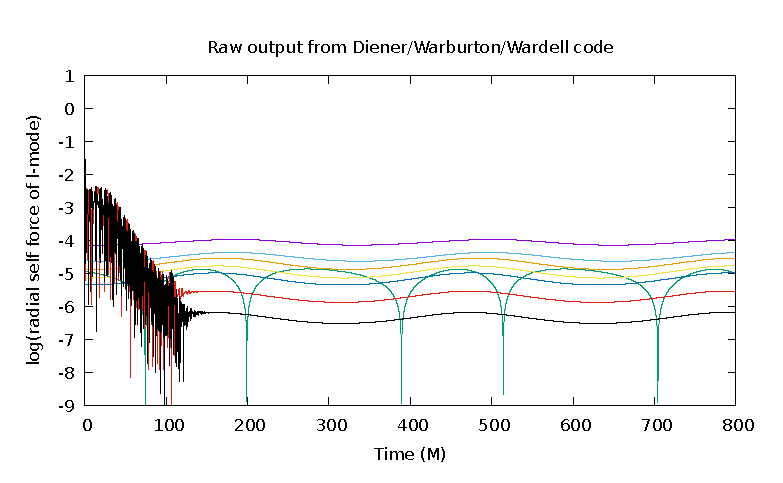
\includegraphics{rawRadialSelForceModes}
  \caption{Raw output of Diener, Warburton, and Wardell code for DG order 44. Radial self force.}
\end{figure}

\begin{figure}
  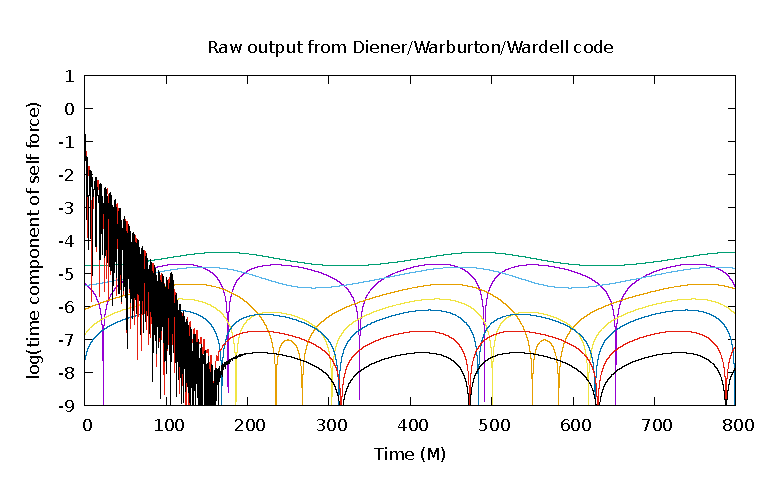
\includegraphics{rawTimeSelfForceModes}
  \caption{Raw output of Diener, Warburton, and Wardell code for DG order 44. Time component of the self force.}
\end{figure}

\begin{figure}
  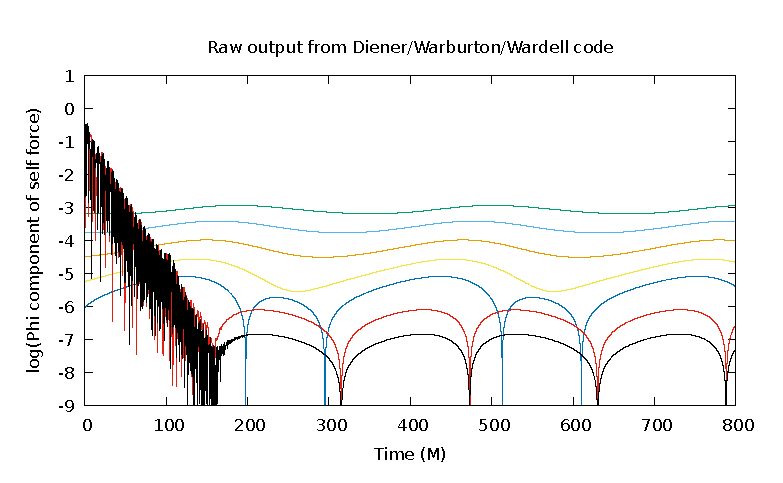
\includegraphics{rawPhiSelfForceModes}
  \caption{Raw output of Diener, Warburton, and Wardell code for DG order 44. Phi component of the self force.}
\end{figure}

